\documentclass[11pt,a4paper]{article}
\usepackage[margin=2.2cm]{geometry}
\usepackage{amsmath, amssymb, amsthm}
\usepackage{graphicx}
\usepackage{booktabs}
\usepackage[hidelinks]{hyperref}
\usepackage{xcolor}
\usepackage{caption}
\usepackage{microtype}
\usepackage{titling}

\setlength{\droptitle}{-1.5cm}

\title{\textbf{QML}}
\author{Kinan Aoukar , Alice Fanny Wimmer, Mykola Savych}
\date{May 2026}

\begin{document}
\maketitle

% ---------------------------------------------------------------------
\section{Introduction}

Quantum machine learning (QML) promises to extend the classical ML toolkit
with new model families, but a working QML pipeline requires answering
a question that has no classical analog: \textit{how do you turn classical
data into a quantum state?} This is the \emph{data encoding} problem, and
the literature is clear that the encoding choice — more than the choice
of ansatz, optimizer, or measurement — dominates the empirical behavior
of variational QML on classical inputs \cite{schuld2021}.

This project compares two encodings — \emph{angle} (one qubit per pixel)
and \emph{amplitude} (pixels packed into amplitudes of a multi-qubit state) —
on a grayscale image classification task. The encodings feed into three
classical heads (MLP, SVM, KAN) plus a logistic-regression baseline, so we
can also test whether encoding effects depend on the downstream model.
A held-out test set, multiple random seeds, and a deployment-noise stress
test were added to make the comparison defensible.

% ---------------------------------------------------------------------
\section{Idea}

\paragraph{Core hypothesis.} If quantum encoding has a useful role to play
on classical data, the difference between encodings should be visible
\emph{and} systematic across models. We hypothesise that:
\begin{enumerate}
    \item On clean data, raw classical features will beat both quantum
        encodings — there is no information advantage to gain from a fixed
        quantum feature extractor.
    \item Encoding choice will dominate model choice: swapping between
        angle/amplitude/raw should move accuracy more than swapping between
        LR/MLP/SVM/KAN.
    \item Amplitude encoding's built-in L2 normalisation will provide
        noise robustness that the classical baseline and angle encoding
        lack.
\end{enumerate}

\paragraph{Physical intuition for angle encoding.} A pixel value $p \in
[0,1]$ is mapped to a rotation angle so that measuring $|1\rangle$ has
probability exactly $p$. Starting from $|0\rangle$ and applying $R_Y(\theta)$,
\[
R_Y(\theta)\,|0\rangle = \cos(\theta/2)\,|0\rangle + \sin(\theta/2)\,|1\rangle,
\quad P(|1\rangle) = \sin^2(\theta/2).
\]
Inverting gives the encoding $\theta = 2\arcsin(\sqrt{p})$, which is what
the experiments below use.

% ---------------------------------------------------------------------
\section{Methods}

\subsection{Pipeline}

The full processing chain is shown in Figure~\ref{fig:pipeline}. Each
MNIST image is downsampled from $28\!\times\!28$ to $4\!\times\!4$ via
$7\!\times\!7$ average pooling, then routed into one of the two quantum
encodings. The encoded state is passed through a fixed ring of CNOTs
and read out via single-qubit $\langle Z_i\rangle$ measurements; the
resulting feature vector feeds a classical classifier head. Only the
classical head is trained — the quantum stage holds no trainable
parameters, so any difference in accuracy across encodings is
attributable to the encoding itself.

\begin{figure}[!htbp]
\centering
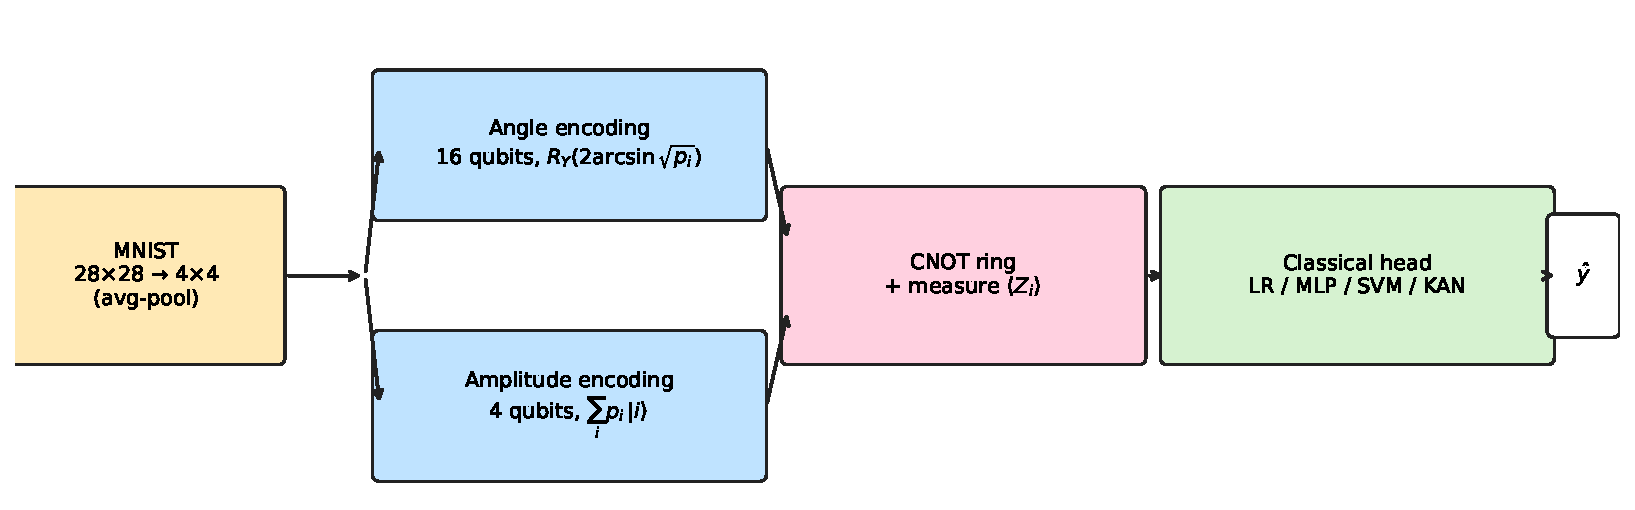
\includegraphics[width=\linewidth]{figs/pipeline.pdf}
\caption{End-to-end pipeline. The same image flows into both encodings;
the classical model is trained on the resulting measurement vector. The
quantum stage (encoding + CNOT ring + readout) contains no trainable
parameters — only the classical head is trained.}
\label{fig:pipeline}
\end{figure}

\subsection{Encodings}

\paragraph{Angle.} For each of the 16 downsampled pixels $p_i$, apply
$R_Y(2\arcsin\sqrt{p_i})$ to qubit $i$. Then a single ring of CNOTs
entangles neighbours. Measurement returns the 16-dimensional vector
$(\langle Z_0\rangle, \dots, \langle Z_{15}\rangle)$.

\paragraph{Amplitude.} L2-normalise the 16-pixel image vector and load it
into the $2^4 = 16$ amplitudes of a 4-qubit state via Möttönen state
preparation \cite{mottonen2005}. Apply the same CNOT ring, then measure
$(\langle Z_0\rangle, \langle Z_1\rangle, \langle Z_2\rangle,
\langle Z_3\rangle)$. The encoding is exponentially more compact in qubit
count but inherently lossy in feature count.

\begin{figure}[h]
\centering
\begin{minipage}{0.49\linewidth}\centering
    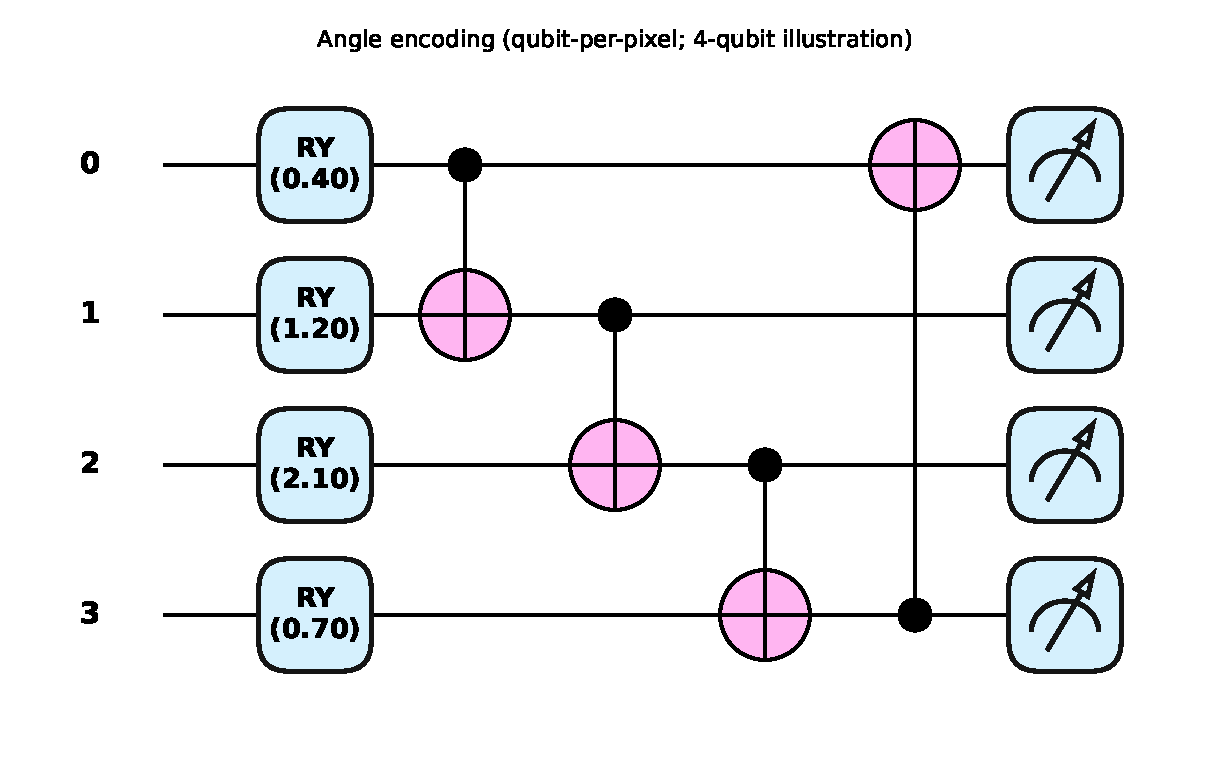
\includegraphics[width=\linewidth]{figs/circuit_angle.pdf}
\end{minipage}\hfill
\begin{minipage}{0.49\linewidth}\centering
    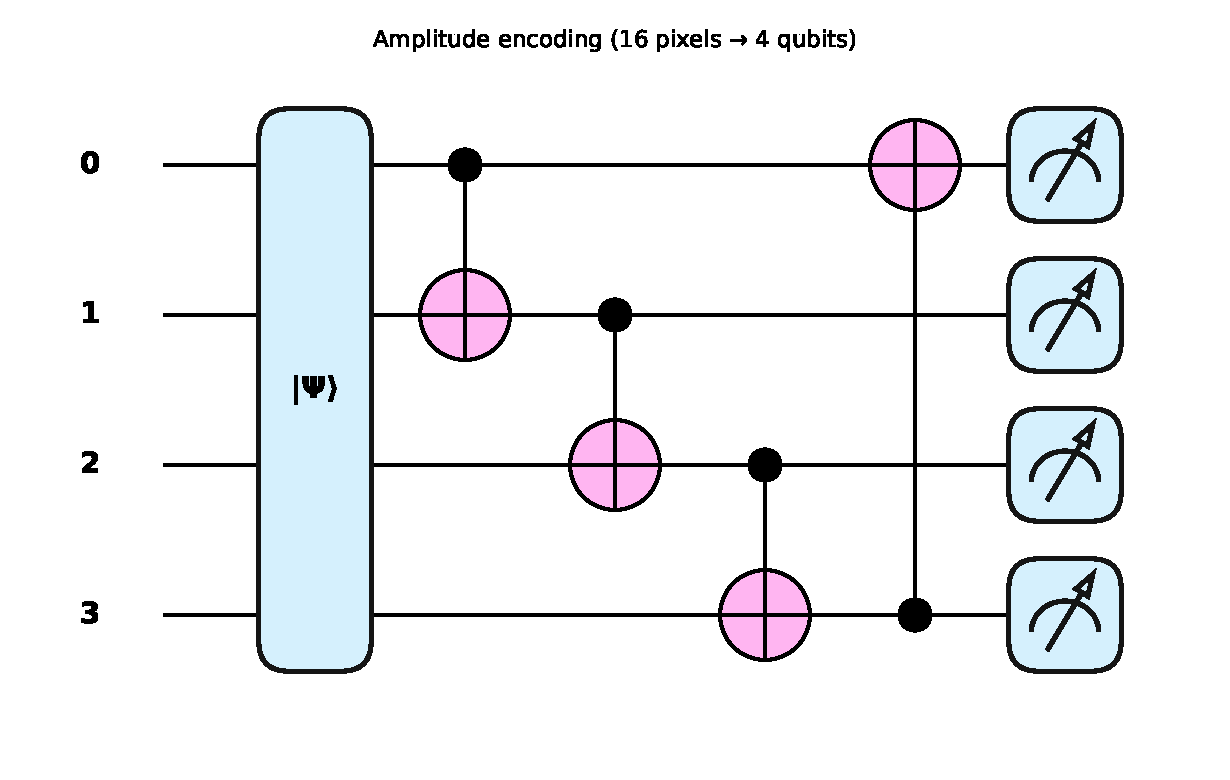
\includegraphics[width=\linewidth]{figs/circuit_amplitude.pdf}
\end{minipage}
\caption{The two encoding circuits, shown at 4-qubit / 16-amplitude scale
for clarity. The experiments use the same structure scaled to 16 qubits
(angle) or 4 qubits (amplitude).}
\label{fig:circuits}
\end{figure}

\subsection{Classical heads}
Each head receives the measurement vector and is trained from scratch:
\begin{itemize}
    \item \textbf{LR} — multinomial logistic regression (L-BFGS).
    \item \textbf{MLP} — one hidden layer of 32 ReLU units, Adam, early
        stopping.
    \item \textbf{SVM} — RBF kernel, $C = 1$.
    \item \textbf{KAN} — single-layer Kolmogorov–Arnold network with 8
        Gaussian RBF basis functions per input edge, trained as multinomial
        logistic regression over the basis-expanded features. This is the
        QuKAN paper's structural definition \cite{kiefer2025} adapted to
        a classical solver.
\end{itemize}

\subsection{Data}
MNIST training images (Kaggle Digit Recognizer split, 42{,}000 samples).
We use a stratified subsample of 3{,}000 images for training (300 per
digit), downsampled $28\!\times\!28 \to 4\!\times\!4$ via $7\!\times\!7$
average pooling. A sealed hold-out test set of 1{,}000 fresh images
(disjoint indices) is encoded once and used only for the final
evaluation.

\subsection{Evaluation}
For each combination of (encoding $\times$ model), the model is trained
on the full 3{,}000-sample training set under three random seeds. We
report two test conditions:
\begin{enumerate}
    \item \emph{Clean test}: held-out test features unchanged.
    \item \emph{Noisy test ($\sigma = 0.2$)}: Gaussian noise added to the
        held-out test features only — the model trained on clean data sees
        corrupted input at evaluation time (a deployment-noise stress test).
\end{enumerate}
Accuracy and macro-F1 are reported, averaged over seeds.

% ---------------------------------------------------------------------
\section{Results}

\begin{figure}[h]
\centering
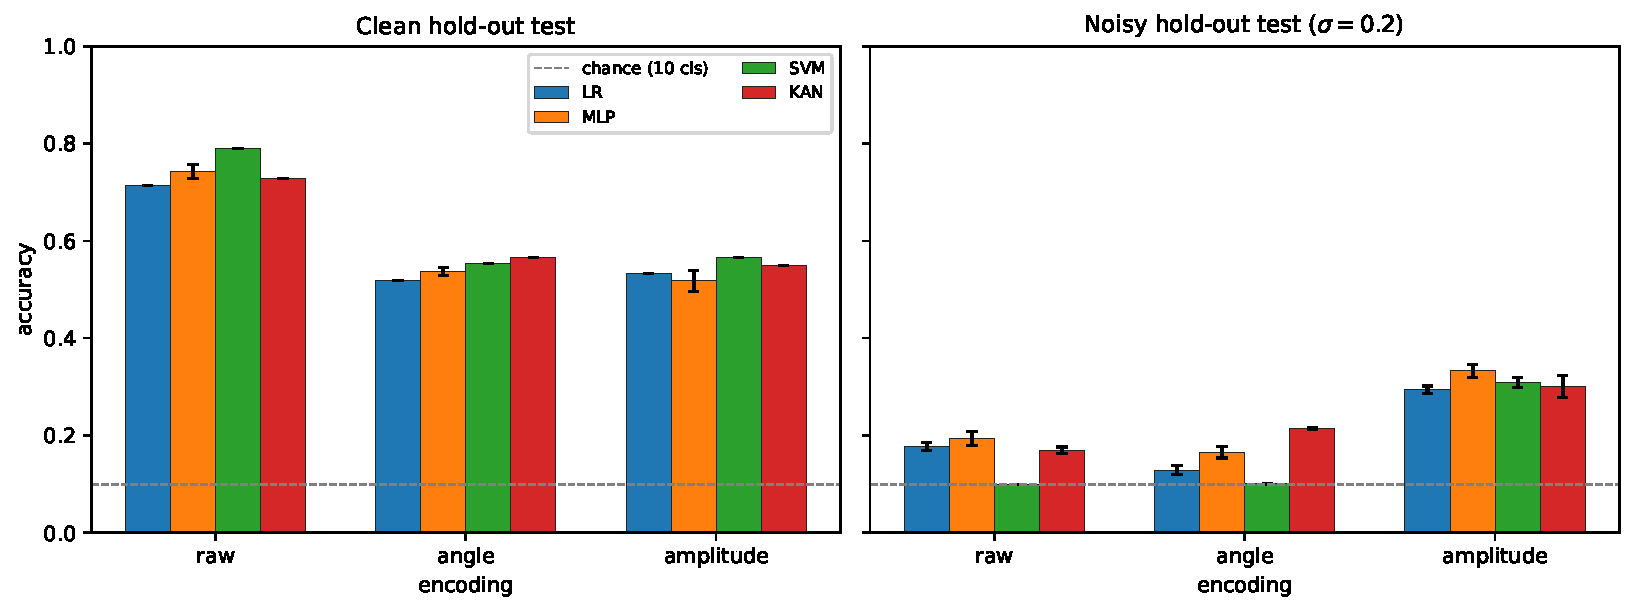
\includegraphics[width=\linewidth]{figs/main_results.pdf}
\caption{Hold-out test accuracy across encodings and classical heads.
Left: clean test. Right: noisy test ($\sigma = 0.2$). Error bars are the
standard deviation across three random seeds. Dashed line is chance
(10\%, 10-class problem).}
\label{fig:results}
\end{figure}

\paragraph{Clean test.}
The raw classical baseline wins decisively — SVM on raw pixels reaches
\textbf{78.9\%} accuracy. Both quantum encodings underperform: amplitude
clusters around 52–57\%, angle around 52–57\%. Within each encoding,
SVM is consistently the strongest model, but the gap to LR/MLP/KAN is
only 2–6 points. The dominant effect is encoding choice, not model choice
(Hypothesis 2 confirmed).

\paragraph{Noisy test.}
The picture inverts dramatically under deployment noise. The raw +
SVM cell collapses to \textbf{10.0\%} accuracy — exactly chance on a
10-class problem. Angle encoding fares no better (10--21\%). \emph{Amplitude
encoding is the only configuration that retains useful accuracy under
noise}, with a 29--33\% range across models (Figure~\ref{fig:results},
right).

\begin{figure}[h]
\centering
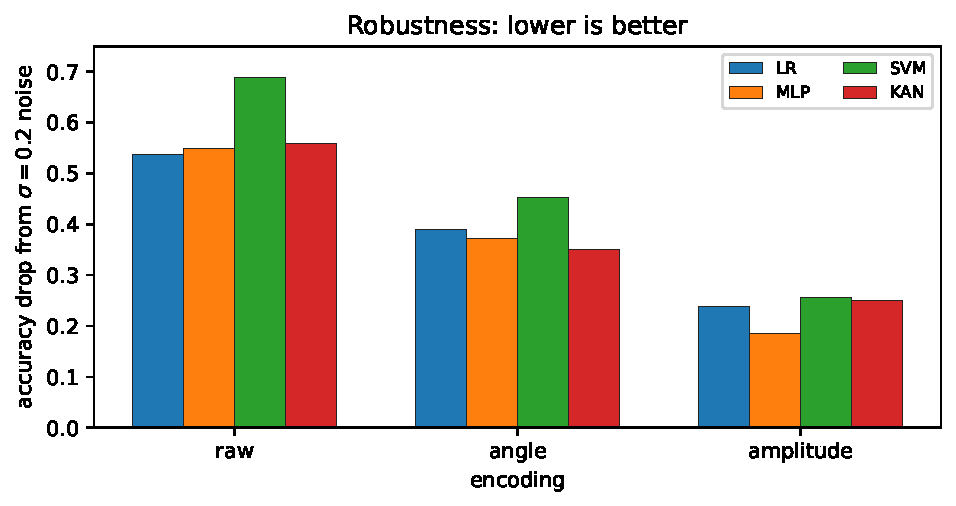
\includegraphics[width=0.72\linewidth]{figs/robustness.pdf}
\caption{Accuracy drop from clean to $\sigma=0.2$ noisy hold-out test,
$\Delta_{\mathrm{acc}} = \mathrm{accuracy}_{\mathrm{clean}} -
\mathrm{accuracy}_{\mathrm{noisy}}$. Lower is better.}
\label{fig:robustness}
\end{figure}

\paragraph{Robustness summary.}
The drop in accuracy from clean to noisy test
(Figure~\ref{fig:robustness}):
\begin{center}
\begin{tabular}{lcc}
\toprule
Encoding & Clean (mean) & Drop ($\sigma=0.2$) \\
\midrule
Raw       & 74\,\% & $-58$ pp \\
Angle     & 54\,\% & $-39$ pp \\
Amplitude & 54\,\% & $-23$ pp \\
\bottomrule
\end{tabular}
\end{center}

Amplitude encoding is roughly \emph{three times more noise-robust} than
either alternative. Its built-in L2 normalisation, plus the fact that
each output feature is a sum over many input pixels, gives the encoding
a free denoising property that the per-pixel angle encoding does not
share (Hypothesis 3 confirmed).

% ---------------------------------------------------------------------
\section{Conclusion}

\paragraph{What we found.}
On a strict hold-out test of MNIST images:
\begin{itemize}
    \item Without noise, fixed quantum feature extraction loses accuracy
        relative to a classical baseline by 20--30 absolute points. There
        is no encoding magic in the clean-data regime.
    \item Encoding choice dominates model choice. Swapping
        raw / angle / amplitude moves accuracy by 20+ points; swapping
        LR / MLP / SVM / KAN moves it by less than 10.
    \item Under deployment noise ($\sigma = 0.2$), amplitude encoding
        \emph{outperforms} the raw classical baseline by roughly 20 points
        of accuracy. The reversal is large and consistent across all four
        classical heads.
\end{itemize}

\paragraph{Why amplitude wins under noise.}
The L2 normalisation in amplitude encoding makes the encoded state
invariant to the overall brightness of the input. Combined with the
$16\!\to\!4$ feature compression — each output observable is a sum over
eight amplitudes — this constitutes a quantum-native form of
\textit{denoising-by-aggregation}. Angle encoding, by contrast, places
one qubit per pixel, so per-feature noise is essentially per-pixel
noise.

\paragraph{Limitations.}
The quantum stage uses no trainable parameters; a trainable circuit
(variational classifier) could close some of the clean-data gap but
would conflate encoding effects with ansatz expressivity. The downsampling
to $4\!\times\!4$ throws away most of MNIST's information; ceiling
accuracies of $\sim$80\% reflect that, not encoding quality. Noise was
injected at the post-measurement feature level, not the input pixel level
— defensible for hardware-noise modelling but not the same as physical
sensor noise.

\paragraph{Next steps.}
Three follow-ups are most likely to sharpen the picture: (i) sweep
noise levels $\sigma \in \{0.05, 0.1, 0.2, 0.3, 0.5\}$ to turn the
robustness number into a curve; (ii) enrich the angle-encoding readout
to include $\langle X_i\rangle$ and $\langle Y_i\rangle$ (and two-qubit
correlators) so the encoding actually uses all of the quantum state
information available; (iii) compare amplitude encoding's noise
robustness against a classical compressed-representation baseline (PCA
to 4 dimensions, autoencoder bottleneck) to establish whether the
robustness is genuinely quantum-specific or simply a consequence of
dimensionality reduction.

% ---------------------------------------------------------------------
\begin{thebibliography}{9}
\bibitem{kiefer2025}
M.~Kiefer-Emmanouilidis et al.,
\textit{QuKAN: A Quantum Circuit Born Machine Approach to Quantum
Kolmogorov Arnold Networks}.
Scientific Reports 15, 35239 (2025). DOI: 10.1038/s41598-025-22705-9.

\bibitem{schuld2021}
M.~Schuld,
\textit{Quantum Machine Learning Models are Kernel Methods}.
arXiv:2101.11020 (2021).

\bibitem{mottonen2005}
M.~Möttönen, J.~J.~Vartiainen, V.~Bergholm, and M.~M.~Salomaa,
\textit{Transformation of quantum states using uniformly controlled
rotations}.
Quantum Information \& Computation 5, 467 (2005).
\end{thebibliography}

\end{document}
